\chapter{Basic operations and settings}\label{chap:basic}

Now, I suppose that the reader can run the program successfully and get the first window. Formerly, in the first version of \textsc{Pāli\,Platform}, all working areas are integrated into one window. From version 2 onward, the program has multiple windows. So, you will see many windows doing various jobs. There are two kinds of window: singleton and multi-instance. The former has only one instance in the program's lifetime (About dialog, for example), whereas the later can have multiple instances (Dictionaries window, for example). Let us start with the main window.

\section{Main window}

The main window is a mandatory singleton. You only have one main window when you run the program. And you should not start the program multiple times from the same directory. It seems you cannot do so because of the conflict of shared resources.

There are three parts in the main window: the menu bar, the main tool bar, and tabs of some working areas (see Figure \ref{fig:main-window}). The first two parts are familiar to most computer users. Every button in the tool bar has its counterpart in the menu. They are selected to show here because they are used a lot.

The third part is the big area below those two. There are six fixed tabs of the most used tools: TOC Tree, Document Finder, Lucene Finder, Term Lister, Dictionaries, and Editor. These tabs are always there, no more no less. Each tab can be opened as new multiple windows using the menu or the tool bar. When a new window is created, it works separately from the main tab area. For referencing, therefore, we will call these six tabs as the main TOC Tree, the main Document Finder, and so on.

On the first start, except the Editor, the content of these tabs are not loaded. If you want to use one of them, hit the Load button in each tab.

\section{Common tool bar}

Every working tab, also every opened window, has its own tool bar that has a part in common (see Figure \ref{fig:common-toolbar}).

\begin{figure}[!hbt]
\centering

\includegraphics[width=0.8\linewidth]{images/common-toolbar.png}\\
\caption{The common local tool bar}
\label{fig:common-toolbar}
\end{figure}

Each button in the common tool bar, has the same function in all windows (but its behavior may be different). The description of all these is shown in Table \ref{tab:common-toolbar}.

\begin{table}[!hbt]
\centering
\caption{Buttons of the common tool bar}
\label{tab:common-toolbar}
\bigskip
\begin{tabular}{ll} \toprule
{\faSix \symbol{"F186}} & Switch between light and dark theme \\
{\faSix \symbol{"F056}} & Decrease font size \\
{\faSix \symbol{"F021}} & Reset font to normal size \\
{\faSix \symbol{"F055}} & Increase font size \\
{\faSix \symbol{"F031}} & Change font \\
{\faSix \symbol{"F56D}} & Save data as text \\
{\faSix \symbol{"F0C5}} & Copy data as text \\
\bottomrule
\end{tabular}
\end{table}

When you change theme by the tool bar, it changes only that instance. If you click {\faSix \symbol{"F186}} button in the main tabs, the whole main window is changed. This change is not persistent. If you want permanent theme change, use menu Options > Global\,theme instead. Other buttons are intuitively understandable, but read more about fonts in its section below. Another common button you can see here and there is help ({\faSix \symbol{"F059}}) button. When clicked, the related help of that part will show up.

\section{Fonts and problems}\label{sect:fonts}

The users will not feel the significance of fonts and their problems until they read or edit a Pāli text. However, you should know this before you find out yourself that things do not always go as you expect.

Fonts used in the program have two kinds: embedded and external. The former has nothing to do with the users. You may be able to select one of them, but they cannot be changed or removed. This includes \emph{DejaVu}\footnote{\url{dejavu-fonts.github.io}} font family (Serif, Sans Serif, and Mono space) and icon fonts. In \textsc{Pāli\,Platform\,3}, \emph{Paduak\,PP}\footnote{The original Paduak font is taken from \url{fonts.google.com/specimen/Padauk}.} font (modified) is also embedded for using with Myanmar script. So, when applicable, you can always choose either \emph{DejaVu Serif} or \emph{DejaVu Sans} or \emph{DejaVu Sans Mono}. These fonts should have no problem in most running environment.

Problems mostly come from other scripts than Roman. That is why external fonts are needed. The idea is simple: put your font files (TTF) in folder \texttt{fonts} at the program's root and restart the program. You should add two files: one for regular face, another for bold face. If only regular face is added, you will see only regular text, no bold, in Pāli documents.

Not every font is usable, however. For displaying Pāli Roman, you must have a Unicode font with \emph{Latin Extended Additional} block (not every Unicode font has it).

For other scripts, I only added \emph{Noto\,Sans\,Myanmar\,PP}\footnote{The original Noto fonts can be found at \url{github.com/notofonts/noto-fonts}.} (modified) font for an alternative use with Myanmar script. For other scripts, except Myanmar, you have to find a suitable font yourselves (or leave it to the system, if you are lucky). Here is a warning: Not all fonts work as expected. Some fonts may look different in different environment, and some may look weird in certain machines.

When problems related to external fonts occur, one solution you can do is just delete the external fonts. If your system has proper fonts installed, you can delete fonts provided in the font folder (or move them away). Then, the program will use a system font instead as a fallback, currently set to \emph{Sans}.

\boxnote{In \textsc{Pāli\,Platform\,3}, Myanmar script is treated so differently that it needs a custom font to show. Other Myanmar fonts that are not provided by the program will fail to display the text correctly.\\
\hspace{5mm}This is mostly about a Java technical problem. Due to the lack of a firm standard, Java cannot handle Myanmar characters correctly. To solve this problem ad hoc, I have to program the Myanmar script conversion manually to correct the display and use a modified font.\\
\hspace{5mm}Yet the Myanmar display is far from perfect. A new solution may come up in a next version of the program. Now it is just enough for students to learn Myanmar script by the program.\\
\hspace{5mm}\caveat Do not copy a portion of text in Myanmar script and paste it in another program.
}

\section{Pāli input}\label{sect:pali-input}

Typing in Pāli characters is used throughout the program. So, it is essential that the users have to learn the input method. It is easy, but needs some familiarity. In text fields and text areas that expect Pāli Roman characters, there are 3 modes of input indicated by their symbol: Regular mode (a\blacktriangleright a), Unused-characters mode (x\blacktriangleright ā), and Composite mode (ā\blacktriangleright ā). These three modes can be switched circularly by clicking the symbol button or pressing \texttt{Ctrl-Space}. Pāli input also has detailed settings in Settings window, invoked by menu Options > {\faSix \symbol{"F013}} Settings or {\faSix \symbol{"F013}} button in the main tool bar.

\begin{figure}[!hbt]
\centering
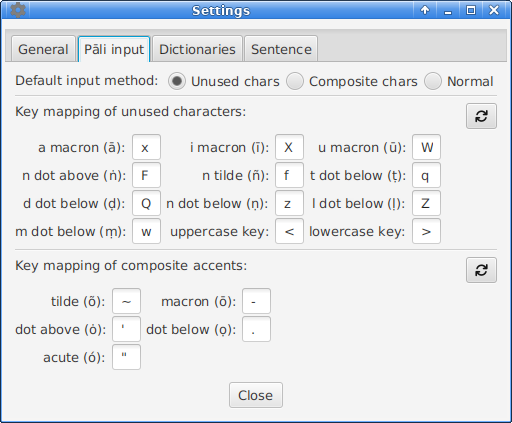
\includegraphics[width=0.9\linewidth]{images/settings-input.png}\\
\caption{Settings for Pāli input}
\label{fig:settings-input}
\end{figure}

\fbox{a\blacktriangleright a} \emph{Regular mode} is the normal state of your computer. As the symbol says, when you type `a' you simply get `a'. You can type in English or other languages supported by your system in this mode.

\fbox{x\blacktriangleright ā} \emph{Unused-characters mode} is a unique and innovative method. This mode utilizes unused English characters for some Pāli letters with diacritics. Here are the program's default mapping: x~=~ā, X~=~ī, w~=~ṃ, W~=~ū, F~=~ṅ, f~=~ñ, q~=~ṭ, Q~=~ḍ, z~=~ṇ, Z~=~ḷ. That is why the symbol says thus: you get `ā' when you hit `x', for example. This mode includes two special keys for making a character under cursor uppercase (<) and lowercase (>). All these keys can be set in Settings (see Figure \ref{fig:settings-input}).

\fbox{ā\blacktriangleright ā} \emph{Composite mode} is the most intuitive way to enter a diacritic mark. Here are the program's presets: $\sim$~=~tilde, -~=~macron, '~=~dot above, .~=~dot below, "~=~acute (see also Figure \ref{fig:settings-input}). For example, when you need `ā' you type `a' followed by `-' immediately. The mapping can be set otherwise in the program's settings. This mode is a little more expensive than the previous one. You need two strokes rather than one, but you do not need to remember the character mapping.

The users can set their preferred method as the default in the program's settings (see Figure \ref{fig:settings-input}).

\boxnote{All user's preferences, such as the global theme, and those in Settings, are saved in an external property file, named \texttt{PaliPlatform3.properties}. This file usually exists in the program's root. If you mess up with the settings, you can return to the original state by just deleting the property file and restart the program.}

\section{Minor concerns}

There are some miscellaneous points that are worth mentioning here, before you make a real use of the program.

\paragraph{(1) Drag-and-drop.} The program supports the drag-and-drop action in various places. For example, a file can be dragged from the system's explorer and drop into the program's editor, or a text portion can be dragged from a system's editor and drop into a Dictionaries window.

There are many possibilities of drag-and-drop. Some look obvious. Some seem likely applicable, but it cannot be done (because of a technical limitation). It will be too fussy to list all of them here. Learning by using is better. If any drag-and-drop action does not work, using copy-and-paste, if applicable, can achieve the same goal in most cases.

\paragraph{(2) Context menus.} Context menus are menus that pop up when you right-click (or left-click in some places) at a certain object. These menus are context-dependent. You have to test and learn by yourself. In many cases, context menus provide more solid functions, than drag-and-drop does.

\paragraph{(3) Sortable tables.} There are a number of tabular results produced by the program. Most of those tables are sortable. It can be done by clicking on the table header of the target columns. The mode of sorting is changed circularly: ascending, descending, and unsorted. A triangle in the header will show up accordingly. Some tables, to which sorting makes no sense, cannot be sorted, though. There are some things to keep in mind. First, most tables are already sorted by a pre-selected criterion. Using a custom sort can disrupt the preset order, in the way that mode of sorting may be shown incorrectly. And second, the sorting is done only on the existing data in the tables. No new retrieval or calculation is applied.

\paragraph{(4) Tooltips.} When you are stuck in the using, try {\faSix \symbol{"F059}} button first. If the help is not available, try reading tooltips by hovering the mouse over an unknown button. Tooltips can be seen in other places as well, such as in a list or table that has truncated data entries.

\paragraph{(5) Databases locked and unlocked.} In \textsc{Pāli\,Platform\,3}, all data\-bases used are created in place. Currently there are three of them: (1) \emph{Dict} DB, for the bundled dictionaries; (2) \emph{PP-DPD} DB, an optimization for DPD data; and (3) \emph{Lister} DB, for Term Lister.

In the first run, all these databases will be created and set to writable waiting for data to be inserted. This is the \emph{unlocked} state ({\faSix \symbol{"F09C}}). You can see the state in the corresponding menus. With this unlocked state, at least in Linux, when the program is finished, it makes the exit linger for a while. To make the exit faster, change the state of databases to \emph{locked} ({\faSix \symbol{"F023}}) instead. This should be done when all data have been created and no more creation is needed. You have to lock all three databases to see the effect. When new data are needed, you can unlock them at any time.
